%% bare_conf.tex
%% V1.4b
%% 2015/08/26
%% by Michael Shell
%% See:
%% http://www.michaelshell.org/
%% for current contact information.
%%
%% This is a skeleton file demonstrating the use of IEEEtran.cls
%% (requires IEEEtran.cls version 1.8b or later) with an IEEE
%% conference paper.
%%
%% Support sites:
%% http://www.michaelshell.org/tex/ieeetran/
%% http://www.ctan.org/pkg/ieeetran
%% and
%% http://www.ieee.org/

%%*************************************************************************
%% Legal Notice:
%% This code is offered as-is without any warranty either expressed or
%% implied; without even the implied warranty of MERCHANTABILITY or
%% FITNESS FOR A PARTICULAR PURPOSE! 
%% User assumes all risk.
%% In no event shall the IEEE or any contributor to this code be liable for
%% any damages or losses, including, but not limited to, incidental,
%% consequential, or any other damages, resulting from the use or misuse
%% of any information contained here.
%%
%% All comments are the opinions of their respective authors and are not
%% necessarily endorsed by the IEEE.
%%
%% This work is distributed under the LaTeX Project Public License (LPPL)
%% ( http://www.latex-project.org/ ) version 1.3, and may be freely used,
%% distributed and modified. A copy of the LPPL, version 1.3, is included
%% in the base LaTeX documentation of all distributions of LaTeX released
%% 2003/12/01 or later.
%% Retain all contribution notices and credits.
%% ** Modified files should be clearly indicated as such, including  **
%% ** renaming them and changing author support contact information. **
%%*************************************************************************


% *** Authors should verify (and, if needed, correct) their LaTeX system  ***
% *** with the testflow diagnostic prior to trusting their LaTeX platform ***
% *** with production work. The IEEE's font choices and paper sizes can   ***
% *** trigger bugs that do not appear when using other class files.       ***                          ***
% The testflow support page is at:
% http://www.michaelshell.org/tex/testflow/

\documentclass[hidelinks,english,conference]{IEEEtran}

\usepackage{graphicx}
\usepackage{grffile}
\usepackage[T1]{fontenc}
\usepackage{babel}
\usepackage{wrapfig}
\usepackage{hyperref}
\usepackage[acronyms]{glossaries}

% \newglossaryentry{aco}{
%     name=ACO,
%     description={Ant Colony Optimization}
% }

\newcommand{\specialcell}[2][c]{%
  \begin{tabular}[#1]{@{}c@{}}#2\end{tabular}}

% \newacronym[longplural={Ant Colony Optimization}]{aco}{ACO}{Ant Colony Optimization}
\newacronym{aco}{ACO}{Ant Colony Optimization}
\newacronym{tsp}{TSP}{Traveling Salesman Problem}
\newacronym{bs}{BS}{Beam Search}

\date{\today}

\pagenumbering{arabic}

% *** MATH PACKAGES ***
\usepackage{amssymb}
\usepackage{amsmath}

\usepackage[linesnumbered,ruled,vlined]{algorithm2e}
\SetKwRepeat{Do}{do}{while}%

\hyphenation{}

\graphicspath{{Pictures/}}
\begin{document}
\title{Ant Colony Optimization: Finding the Longest Path in a Maze}
\author{\IEEEauthorblockN{Armand Maree\\120 178 00}
\IEEEauthorblockA{Department of Computer Science\\
University of Pretoria\\}}
\maketitle

\begin{abstract}
\gls{aco} is a meta heuristic inspired by ant colonies. It is an algorithmic approach to solve combinatorial optimization problems such as the \gls{tsp}. This paper compares the performance of an \gls{aco} to a \gls{bs} algorithm to find the longest path from the entrance to the exit of a maze.
\end{abstract}

\IEEEpeerreviewmaketitle

\section{Introduction}
	\gls{aco} is a meta heuristic inspired by ant colonies \cite{colony2002guest}. The sought after characteristic of the ant colony is the pheromone trailing used between ants to communicate. Another characteristic inherited from the ant colony is the extremely simplistic nature of a single individual, but due to collaboration between these simple individuals an intelligent "hive mind" can emerge.\\
    
    Pheromone trails are laid down by the ants to indicate the path that they have traveled on. These pheromone trails are then used by other ants to guide them to food sources found by other ants. The idea is that the more pheromone is present on a specific path the more likely an ant will be to follow the path. Eventually most ants will be following one path. This path will be very close to a direct path to the food source (in other words, the shortest/most optimal path).\\
    
    This paper will use an \gls{aco} to find the longest acceptable path through a maze stored in an image file. The results of this will be compared to the more classical \gls{bs} algorithm.
    
\section{Background}
	\gls{aco} is usually used to solve problems like the \gls{tsp} which fall in the field of the combinatorial optimization problems. The solutions to these problems are usually found within a finite (although sometimes countably infinite) set of possible solutions \cite{papadimitriou1982combinatorial}. Since finding the most optimal solution can often be extremely hard, an acceptable solution is usually used as the solution.\\
    
    One aspect where \gls{aco} does not completely model the behavior of the actual ant is when pheromones are dropped. The \gls{aco} only drops pheromone as they return to the start. This means that only the paths that actually lead to a solution will have a higher concentration of pheromone on it.
    
\section{Implementation}
	\subsection{ACO Implementation}
	\subsubsection{Maze initialization}
	Once the maze image (a \textit{.bmp} image) is loaded into the program a matrix ($M$) is constructed where $-1$ in position $M_{i,j}$ means that the pixel in row $i$ and column $j$ was black and is thus a wall. All other positions (white pixels) are initialized to $(numRows + numCols) \div 2$. The purpose of $M$ is to firstly keep track of the maze layout but also to keep track of the pheromone concentrations all over the map.\\
    
    The reason non-wall positions in $M$ is initialized to $(numRows + numCols) \div 2$ is to allow every path to always have a chance (although small) to be chosen as a next move. This value is thus the minimum pheromone concentration a non-wall position in $M$ can have.\\
    
    \subsubsection{Choosing a move}
	The \gls{aco} was implemented in such a way that moves leading in the general direction of the exit are less likely to be chosen as the next position to visit in the maze. In other words, if an ant is in the center of a map, and the solution is in the top right corner, then the ant will favor moves that go down or left by multiplying the pheromone concentration of those positions by 1.5. This will cause the ant to be repelled by the exit position and will thus help find the longest path.\\
    
    When an ant has to make a move, the ant uses equation \ref{moveProbabilityEquation} to calculate the probability of choosing a specific move. $\tau_{i,j}$ refers to the pheromone concentration of a specific position, $i$, coming from position $j$ and $ \mathcal{N}_{i}^{k}$ is the set of possibles moves ant $k$ can make from node $i$. After this it choses a pseudo random number, $r\in\left[0,1\right]$, and based on this choses which move to make, by following algorithm \ref{moveChoiceAlgorithm}.
  
  \begin{align}\label{moveProbabilityEquation}
  P_{i,j}= 
  \begin{cases}
  \frac{\tau_{i,j}^{\alpha}(t)}{\sum_{e\in \mathcal{N}_{i}^{k}}\tau_{i,e}^{\alpha}},& \text{if } j \in \mathcal{N}_{i}^{k}\\
  0,              & \text{otherwise}
  \end{cases}\\
  \text{where}, \tau_{i,j}^{\alpha}(t+1) = \tau_{i,j}^{\alpha}(t) + \Delta\tau_{i,j}^{\alpha}(t)\\
  \text{where},  \Delta\tau_{i,j}^{\alpha}(t) = \sum_{k=1}^{n_{k}}\Delta\tau_{i,j}^{k}(t), \alpha=1.0
  \end{align}

    \begin{algorithm}
        \SetAlgoLined
        \caption{Move selection algorithm}\label{moveChoiceAlgorithm}
        possibleMoves = posssible moves ant can make\\
        randomNumber = random number between 0 and 1\\
        sum = sum of all pheromone of moves in possibleMoves\\
        sumCounter = 0\\
        targetCell = null\\
        \Do{targetCell == null and index < possibleMoves.length}{
        		sumCounter += possibleMoves(index) / sum

				\uIf{randomNumber <= sumCounter}{
					targetCell = possibleMoves(index)
				}
                \Else{
                	index++
                }
        }
    \end{algorithm}
    
    \subsubsection{Pheromone dropping}
	Once an ant has found an exit to the maze the ant is "teleported" back to the entrance to the maze and its memory is cleared (i.e. the path it followed and its avoid list, see section \ref{loopDetection}, is reset). Each position the ant visited gets a pheromone increase by following equation \ref{pheromoneUpdate}. In oder to prevent over saturation of a particular path, the maximum amount of pheromone, $\tau_{max}$, that a specific position can have is limited to $numRows * numCols$. 
    \begin{equation}
    	\label{pheromoneUpdate}
        \begin{split}
          \Delta\tau_{i,j}^{k}(t) = L_{k}\\
          \text{where}, L_{k} \text{ is the total length}\\ \text{of the path that ant } k \text{ found.}
        \end{split}
    \end{equation}
    Some paths found early on might not be very good paths and it would be more advantages if these paths play less of a roll the longer the algorithm runs for. This was accomplished by using pheromone evaporation.  After each iteration the pheromone of each position of the maze is updated using equation \ref{evaporationEquation} where $\rho=0.01$.
      \begin{align}\label{evaporationEquation}
  \tau_{i,j}= 
  \begin{cases}
		(1-\rho) \times \tau_{i,j} ,& (1-\rho) \times \tau_{i,j} \geq \tau_{min}\\
  		\tau_{min},              & \text{otherwise}
  \end{cases}
  \end{align}
  
    \subsubsection{Loop detection\label{loopDetection}}
	Detecting loops can be done in two ways, either by removing them right at the end after an ant has found a path or on each iteration when the ant choses a move. The latter option was implemented for this assignment.\\
    
    Initially the algorithm was implemented to simply remove loops from the ant's memory as soon as it detects a loop and pretends like the loop never occurred. This option proved to be somewhat successful for small mazes, but inefficient for larger mazes. The reason for this is that the ant can keep moving in circles and possibly take a very long time to escape the loop, hindering progress significantly.\\
    
    The second approach was to rather have the ant back track until it reaches a point where it can chose a move which it has not visited previously. As the ant back tracks it removes the move from its memory and adds it to an "avoidance matrix" (a matrix that indicates what positions should never be visited again). This approach requires more memory than the first approach but it makes up for this with the reduction in computational time.\\
    
    Originally this approach iterated over the path of the ant in order to determine whether the position has been visited before. This, again, proved useful for smaller maps, but if the path became long this process become exponentially expensive. In order to reduce this constant iteration, a matrix system was implemented. Using this matrix it became possible to mark all the positions an ant has visited and thus make use of the random access nature of arrays in order to speed up the loop detection process. This matrix and the avoidance matrix was combined to reduce memory.
    
    \subsubsection{Stopping conditions}
	For this assignment, the \gls{aco} will run until the first path to the exit is found. Once this first path has been found the algorithm will be allowed to run for another $MAX(2\times previousSolutionIteration, 10000)$ iterations.\\
    
    \subsubsection{Optimizations \label{acoOptimizationSection}}
     In order to reduce the usage of computer memory, ants move in ways that allow them to skip positions that will not require any decision making. For instance, if an ant is located at position 1 in figure \ref{moveSkipImage} then the ant will chose its next move as position 2 or 3. This is because any position between any of these points only has one possible move that can follow. Since position 3 requires that an ant changes direction, the ant is required to stop here even though there is only one possible move that can follow.
    \begin{center}
        \begin{figure}
            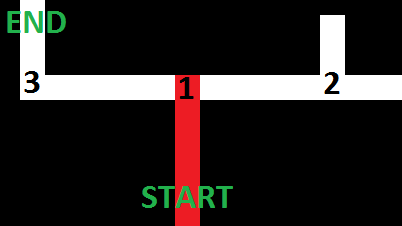
\includegraphics[width=\linewidth]{choices.png}
            \caption{Possible move choices}
		    \label{moveSkipImage}
	    \end{figure}
    \end{center}
    
    When an ant reaches a point where it has no further possible moves, either due to a dead end or due to a loop that might occur, the ant has to back track in order to find another route that it skipped previously. Since there is no real reason why the ant has to physically traverse there, the ant can simply teleport to the last position it decided not to chose. This reduces computational time by avoiding the whole process of moving back on a path that has been previously discovered contains no solution.\\
    
    Mutli-threading has also been used to speed up the searching process. Since the \gls{aco} was run on a 6-CPU system, 6 threads were used. Each thread was responsible for 4 ants to make a total of 24 ants in the colony.\\
    
	\subsection{Beam Search Implementation}
	\subsubsection{Maze Initialization\label{bsMazeInitialization}}
	When the program starts up the maze image is read into a matrix. If a pixel is black, then the cell in the matrix is initialized to $-1$. A white pixel, a.k.a. a path, is initialized to $0$ in the matrix.\\
    
    Each cell in the matrix can contain either the value -1, 0, 1 or 2. The two remaining values (1 and 2), indicates the cell is part of the tree already and the cell is not part of the tree but has been visited, respectively.\\
    
   	\subsubsection{Choosing a move}
	Similar to the way the \gls{aco} was implemented, the \gls{bs} was also implemented in such a way to always favor moves that are further away from the exit. In the \gls{bs} the euclidean distance (equation \ref{euclideanEquation}) was used to determine the distance between any specific cell and the exit to the maze.
    \begin{equation}
   		\label{euclideanEquation}
        r=\sqrt[]{(x_{2} - x_{1})^{2}+(y_{2} - y_{1})^{2}}
    \end{equation}
	Each time the algorithm has to choose which positions it will explore it gathers a list of all possible moves. From these possible moves it choses two and marks their corresponding fields in the matrix (from section \ref{bsMazeInitialization}) as $1$. The remaining fields that is not used will be given the value $2$ in the matrix. The purpose of this is further discussed in section \ref{bsLoopAvoidance}.\\
    
    \subsubsection{Tree details}
	A beam size of 2 was used to construct the a N-ary tree. As the algorithm visits new positions in the maze, a node representing the position is then added as a child to the previously visited node.\\
    
    \subsubsection{Loop avoidance\label{bsLoopAvoidance}}
	\gls{aco} will, if no counter strategy is implemented, get stuck moving in circles when  a loop is encountered. \gls{bs} is more likely to rather terminate without a solution if  a loop is encountered. In order to avoid this occurrence the \gls{bs} will always save any node it did not explore earlier in a temporary list.  Should a situation occur where the \gls{bs} has no more possible moves it simply pops the last two unexplored nodes from the saved list and it carries on like normal. This mechanism ensures that if a path exist \gls{bs} will find it. \gls{bs} is not guaranteed to find the most optimal path since it is possible that the solution is in a subtree that that was previously discarded. \\
    
    \subsubsection{Optimization\label{bsOptimizationSection}}
	Similar to what was done with the \gls{aco}, \gls{bs} also has a jumping behavior when selecting new positions. This saves computational time by avoiding to physically traverse a path that cannot provide ant change in direction. The algorithm simply jumps to the next position that is either an intersection, a dead end, or a turn (or corner).
    
    \section{Research results\label{researchResultsSection}}
	\subsection{ACO results}
	Table \ref{acoResults} shows the times and number of iterations it took to solve each of the mazes. Figures \ref{acoSmall1SolutionImage}, \ref{acoSmall2SolutionImage} and \ref{acoMedium1SolutionImage} shows the paths that were found for mazes Small1, Small2 and Medium1 respectively. As you can note in figure \ref{acoSmall1SolutionImage} and \ref{acoSmall2SolutionImage} the path that is shown clearly indicates the manner in which the ant jumped to next positions as described in section \ref{acoOptimizationSection}.\\
	\begin{table}
    	\centering
        \begin{tabular}{ | c | c | c | }
    		\hline
            Maze Name & \specialcell{Time to Complete\\(min)} & \specialcell{Length of path\\ (num dots in path)}\\
    		\hline
    		\hline
            Small 1 & <1 & 83\\
    		\hline
            Small 2 & <1 & 29\\
    		\hline
            Small-Medium 1 & <1 & 1 581\\
    		\hline
            Small-Medium 2 & <1 & 1 507\\
    		\hline
            Small-Medium 3 & <1 & 716\\
    		\hline
            Small-Medium 4 & <1 & 85\\
    		\hline
            Medium 1 & 377 & 103 419\\
    		\hline
            Medium 2 & 605 & 75 610\\
    		\hline
            Medium 3 & 33 & 5 791\\
    		\hline
            Large 1 & >3205 & N/A\\
    		\hline
        \end{tabular}
        \caption{Time/steps to solve mazes for ACO}
        \label{acoResults}
	\end{table}
  	
    \begin{figure}
    \centering
    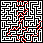
\includegraphics[width=5cm]{Small1_Solution_ACO.png}
    \caption{ACO solution for maze Small1}
    \label{acoSmall1SolutionImage}
    \end{figure}
  	
    \begin{figure}
    \centering
    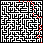
\includegraphics[width=5cm]{Small2_Solution_ACO.png}
    \caption{ACO solution for maze Small2}
    \label{acoSmall2SolutionImage}
    \end{figure}
  	
    \begin{figure}
    \centering
    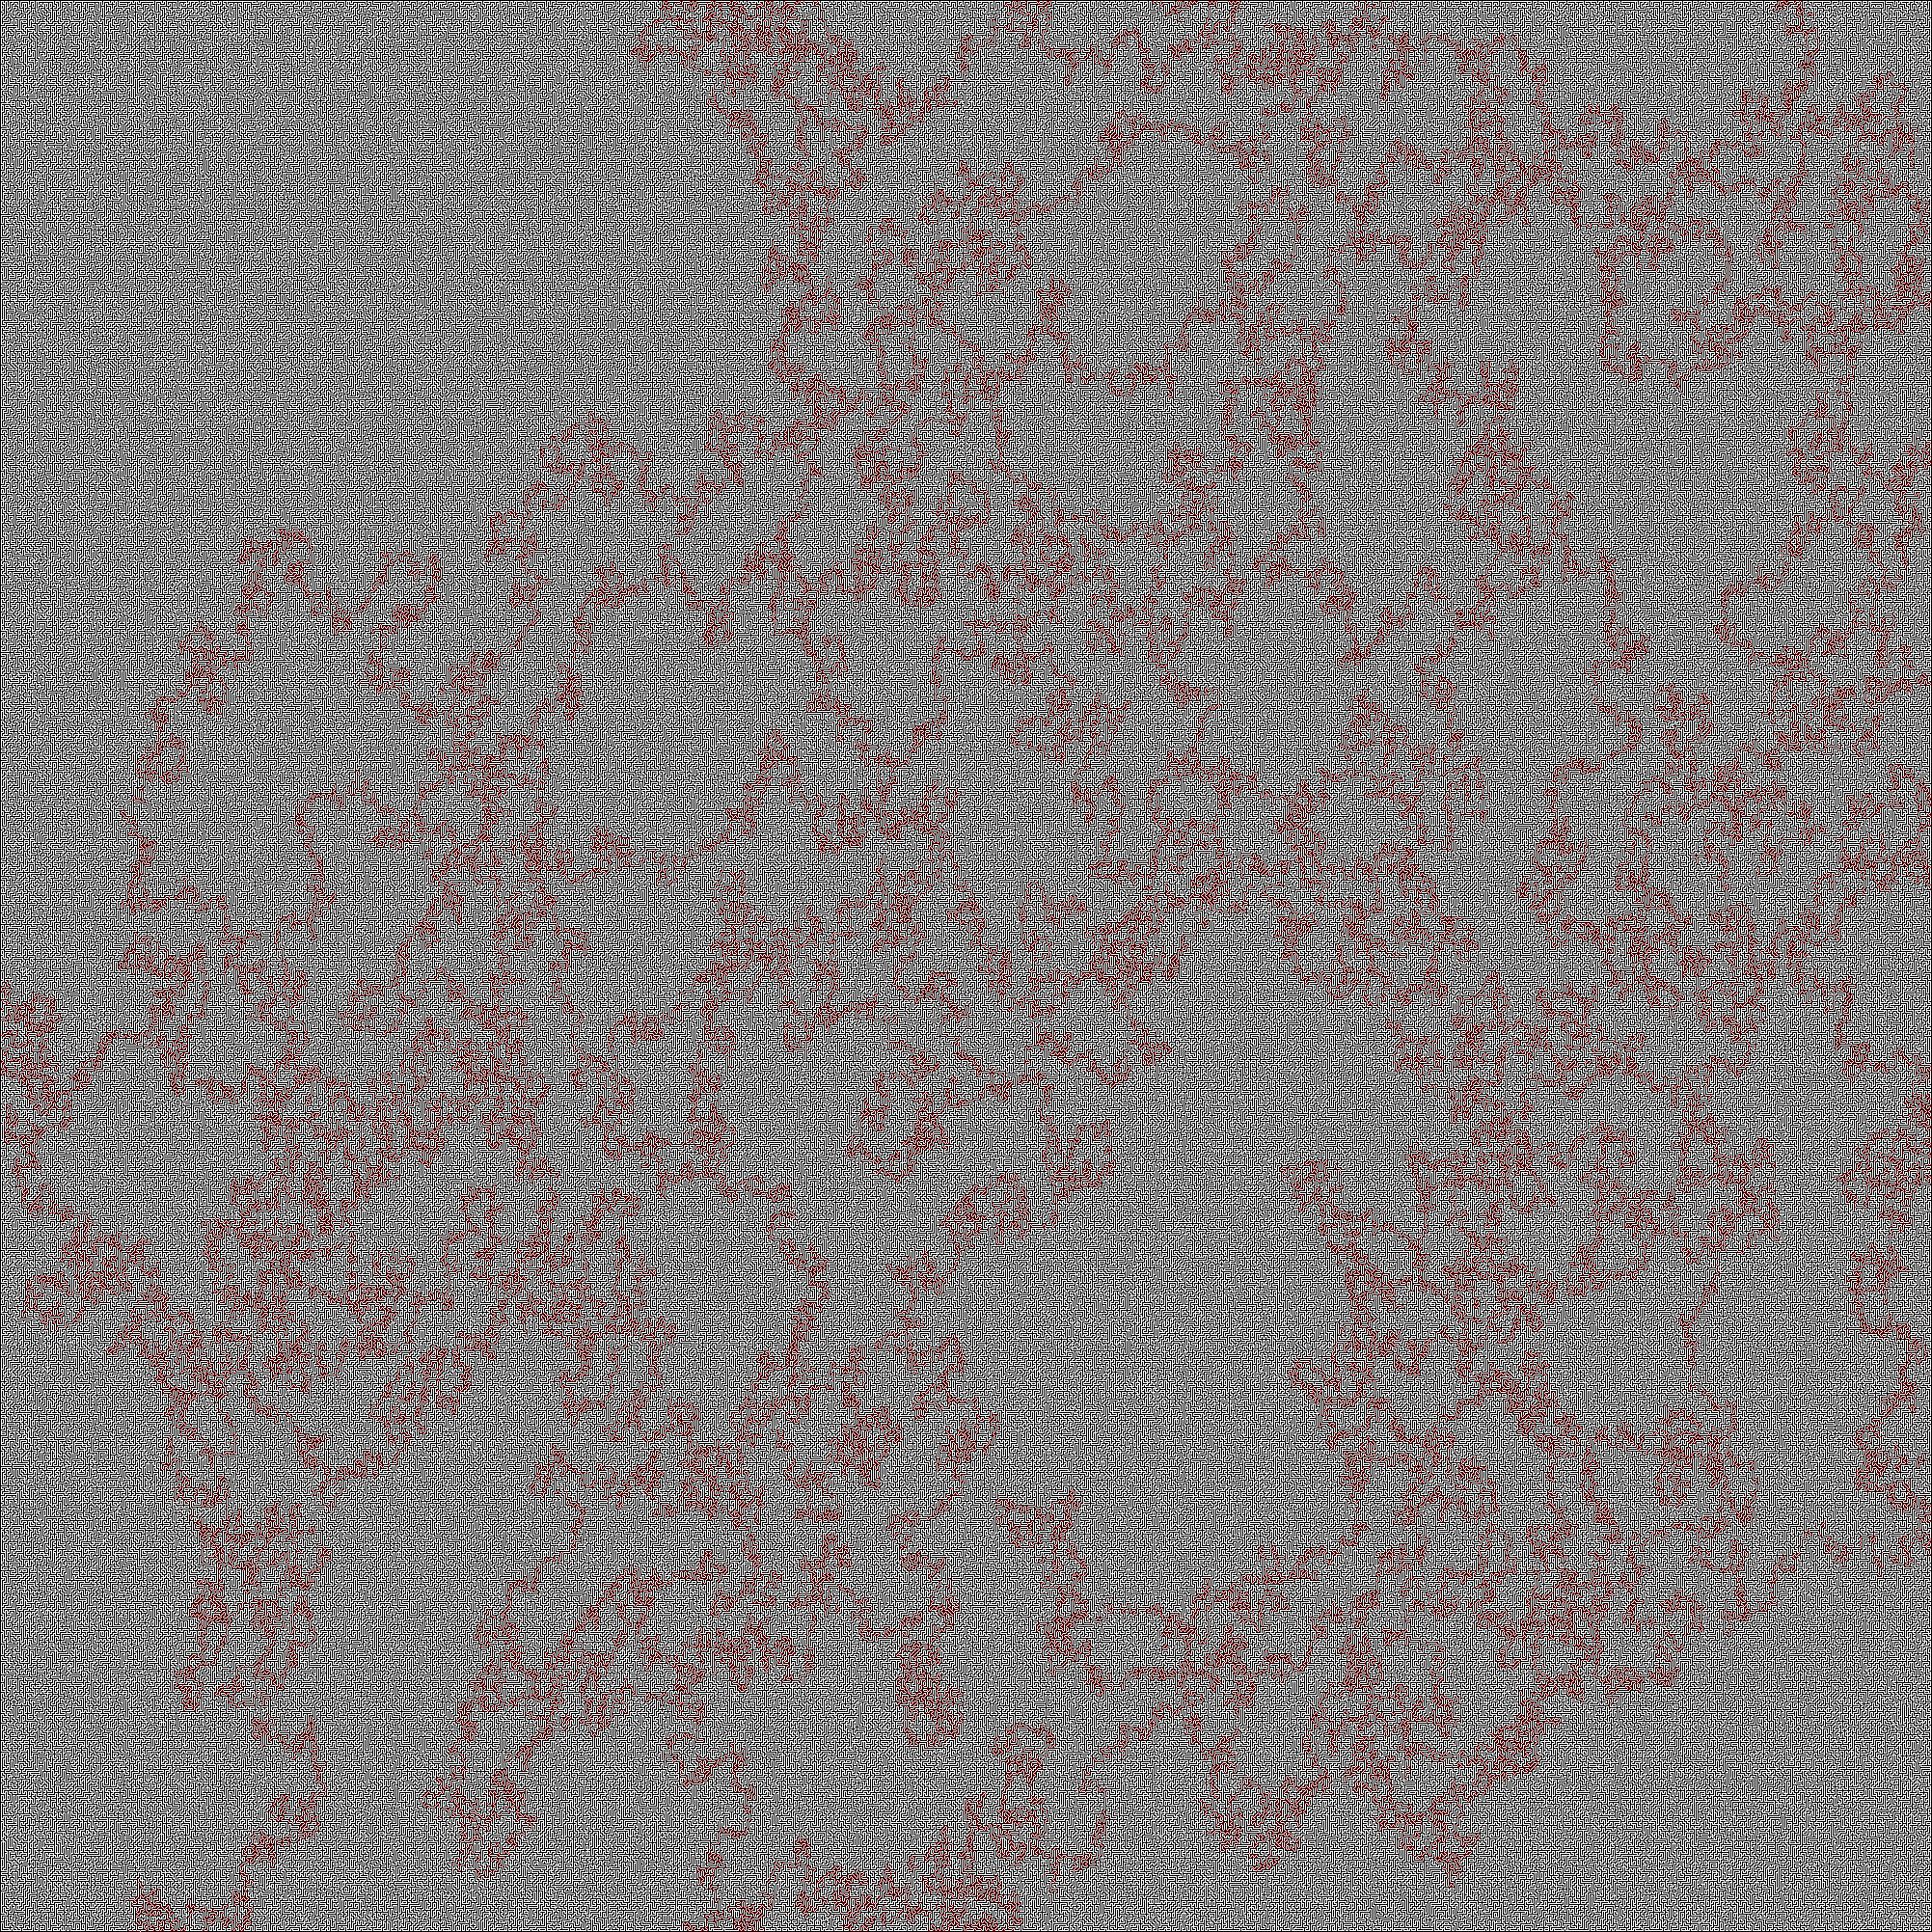
\includegraphics[width=\linewidth]{Medium1_Solution_ACO.png}
    \caption{ACO solution for maze Medium1}
    \label{acoMedium1SolutionImage}
    \end{figure}
    
    Figure \ref{acoSmallMedium2HeatmapImage} faintly shows the different pheromone concentrations that were present during some stage of the \gls{aco} life cycle. More opaque red dots indicate a higher concentration of pheromone where a more transparent dot indicates a lower concentration of pheromone. 
  	
    \begin{figure}
    \centering
    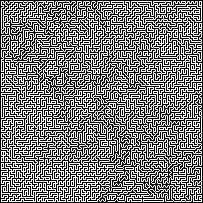
\includegraphics[width=\linewidth]{Small-Medium2_Heatmap_ACO.png}
    \caption{ACO pheromone concentrations for maze SmallMedium2}
    \label{acoSmallMedium2HeatmapImage}
    \end{figure}
      
	\subsection{Beam search results}
	Table \ref{bsResults} shows the results obtained from the \gls{bs} for each of the mazes provided. Figures \ref{bsSmall1SolutionImage}, \ref{bsSmall2SolutionImage} and \ref{bsMedium1SolutionImage} shows the paths that were found for mazes Small1, Small2 and Medium1 respectively. Once again the "jumping" behavior of the \gls{bs} as described in section \ref{bsOptimizationSection} can be seen in figure \ref{bsSmall1SolutionImage} and \ref{bsSmall2SolutionImage}.
	\begin{table}
    	\centering
        \begin{tabular}{ | c | c | c | }
    		\hline
            Maze Name & \specialcell{Time to Complete\\(min)} & \specialcell{Length of path\\ (num dots in path)}\\
    		\hline
    		\hline
            Small 1 & <1 & 71\\
    		\hline
            Small 2 & <1 & 29\\
    		\hline
            Small-Medium 1 & <1 & 1 385\\
    		\hline
            Small-Medium 2 & <1 & 1 530\\
    		\hline
            Small-Medium 3 & <1 & 716\\
    		\hline
            Small-Medium 4 & <1 & 85\\
    		\hline
            Medium 1 & 3 & 123 568\\
    		\hline
            Medium 2 & 2 & 118 059\\
    		\hline
            Medium 3 & <1 & 5 791\\
    		\hline
            Large 1 & 795 & 3 012 138\\
    		\hline
        \end{tabular}
        \caption{Time/steps to solve mazes for BS}
        \label{bsResults}
	\end{table}
  	
    \begin{figure}
    \centering
    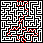
\includegraphics[width=5cm]{Small1_Solution_BS.png}
    \caption{BS solution for maze Small1}
    \label{bsSmall1SolutionImage}
    \end{figure}
  	
    \begin{figure}
    \centering
    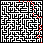
\includegraphics[width=5cm]{Small2_Solution_BS.png}
    \caption{BS solution for maze Small2}
    \label{bsSmall2SolutionImage}
    \end{figure}
  	
    \begin{figure}
    \centering
    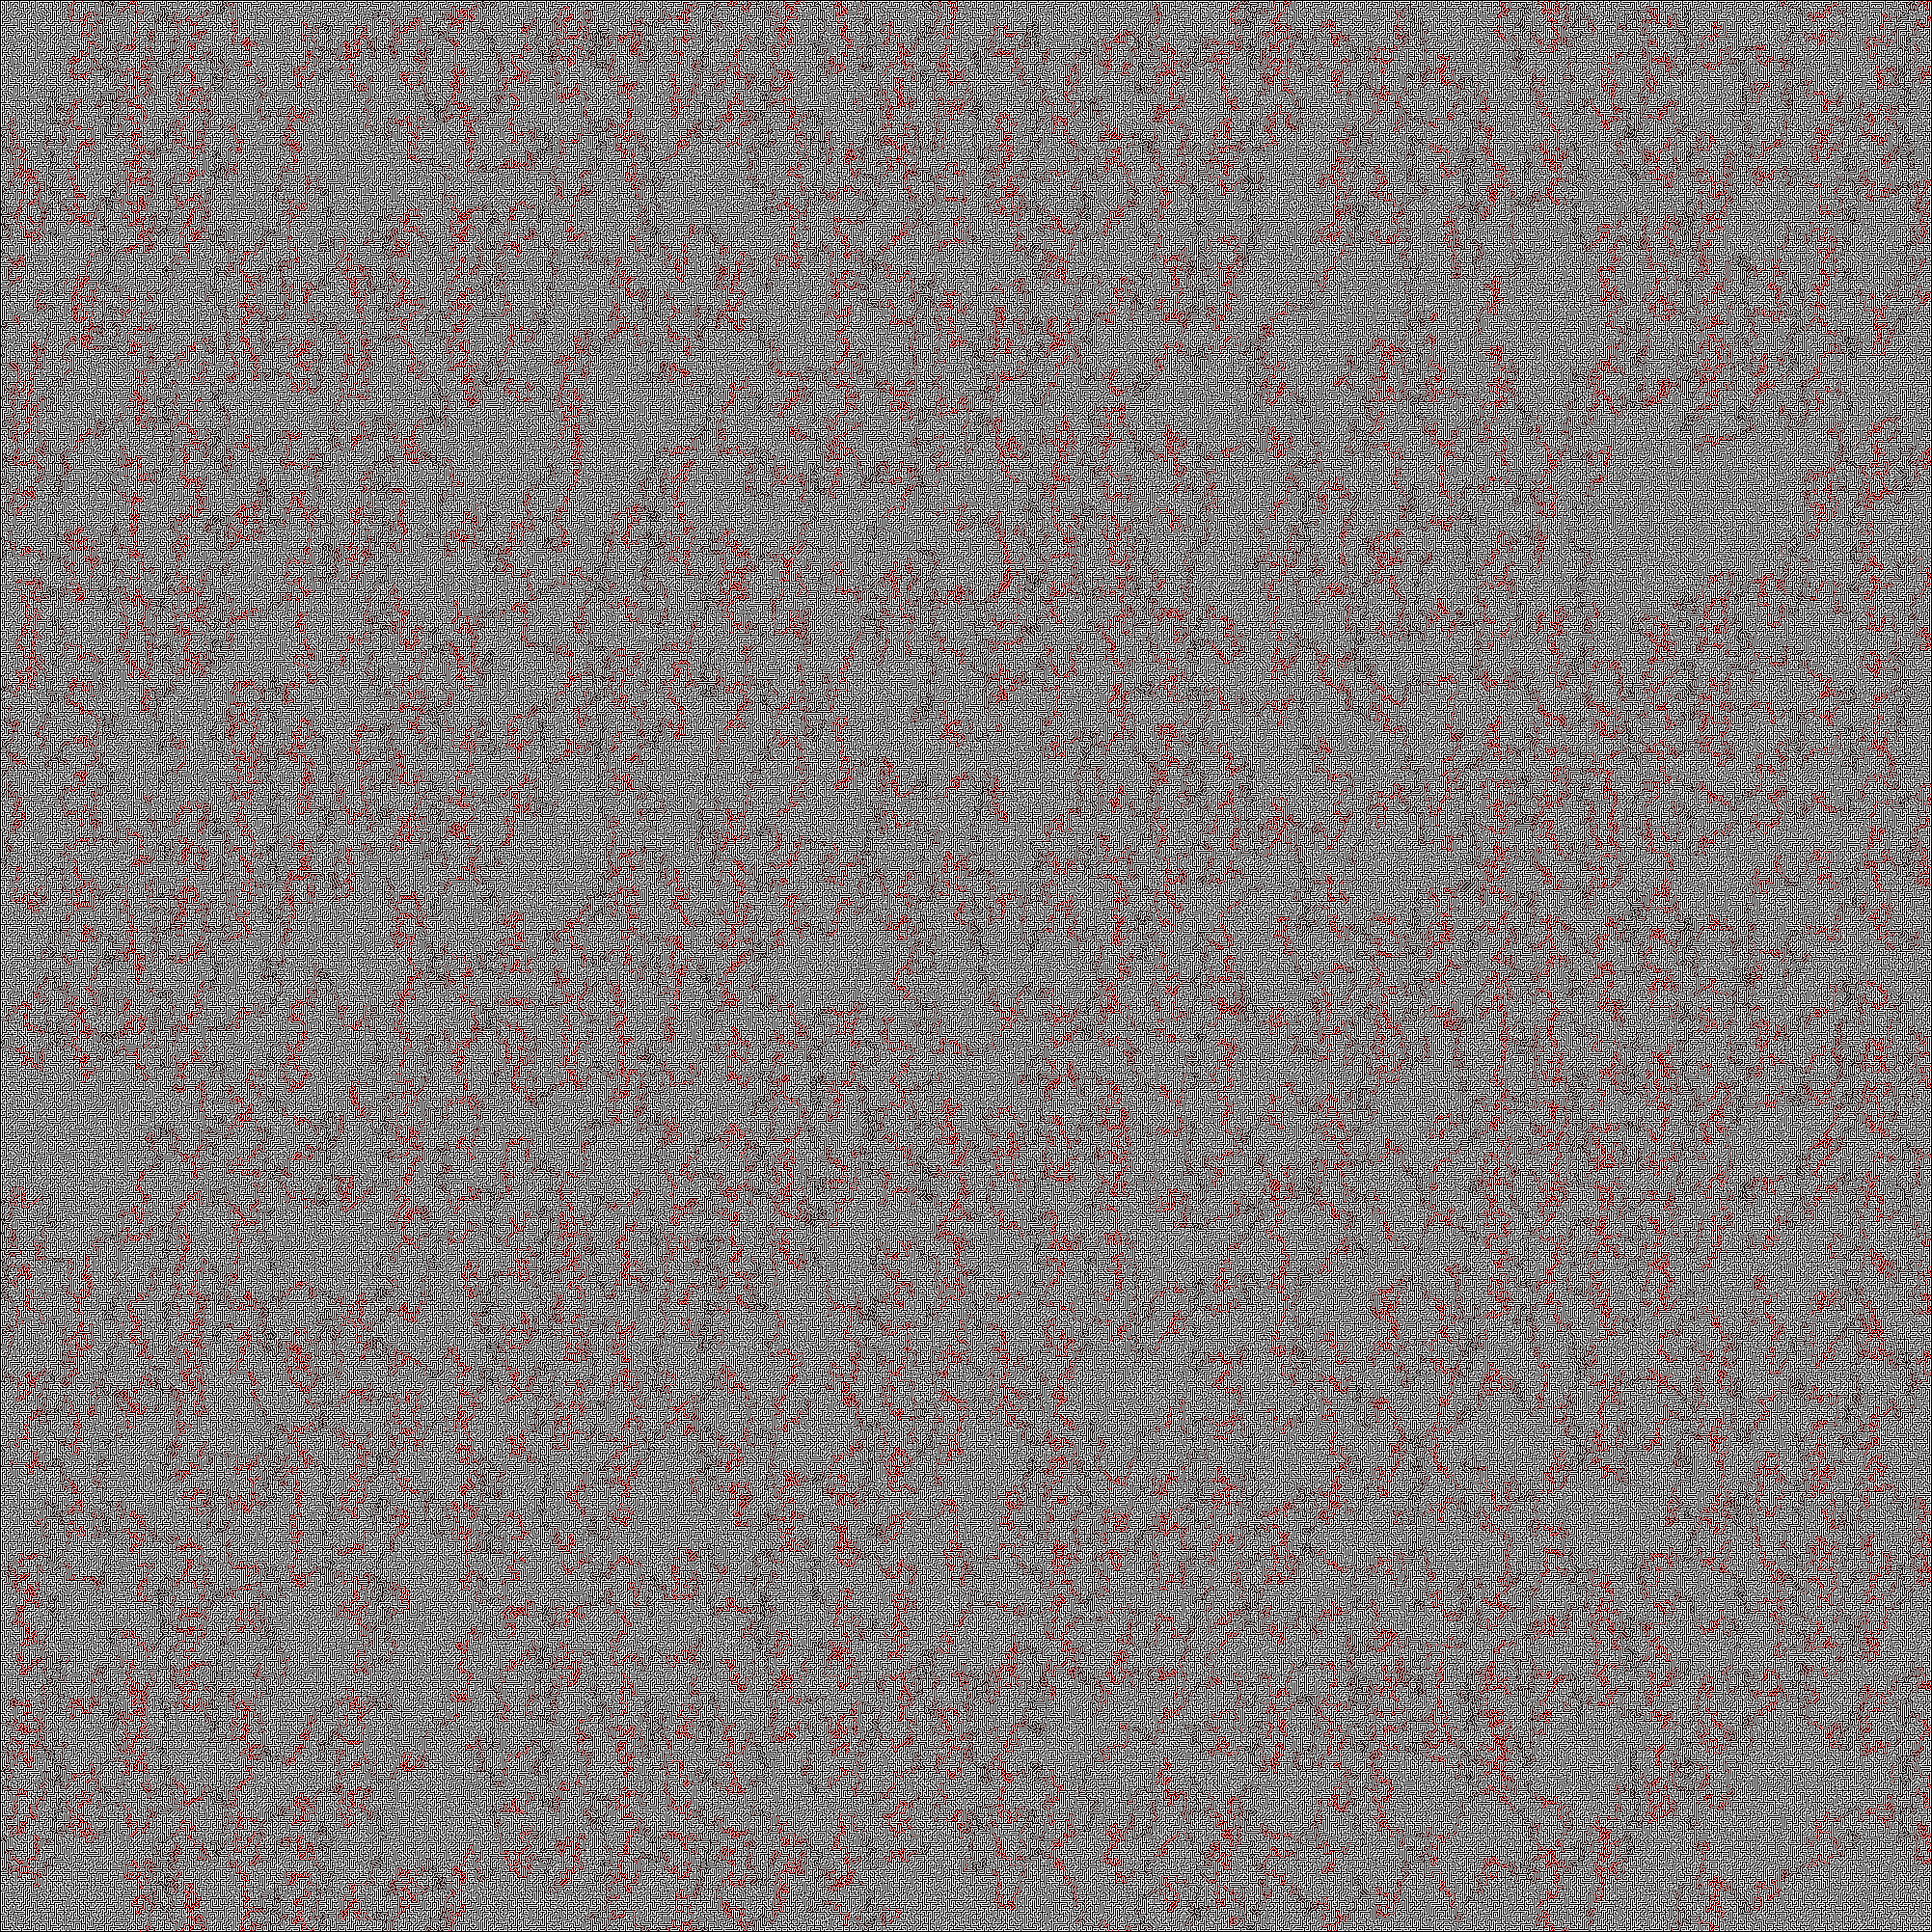
\includegraphics[width=\linewidth]{Medium1_Solution_BS.png}
    \caption{BS solution for maze Medium1}
    \label{bsMedium1SolutionImage}
    \end{figure}
    
    \subsection{Observations}
	Considering the results in section \ref{researchResultsSection} it is clear that \gls{bs} was vastly more superior during the tests. The algorithm is a lot simpler to implement and also takes less time to implement, and it can also find solutions rapidly even though the probability of it discarding  a better solution is higher than with the \gls{aco}. Despite this possibility the \gls{bs} found better solutions than \gls{aco} more often.\\
    
    Another factor to consider is the stochastic nature of the \gls{aco}, during the testing of this algorithm it occasionally found solutions very rapidly (although not as rapidly as \gls{bs}). The results shown in table \ref{acoResults} are the closer to the average time it took to solve the mazes. On the other hand, the \gls{bs} will always produce the same result for a given maze since it does not contain any stochastic component. This can be seen as a negative aspect if the algorithm finds a solution that is very far from the optimal, as it will always in subsequent runs produce this path.\\
    
    Another interesting event to note is that \gls{aco} spends less time to find a solution than it spends on optimizing that solution. The outcome of these results (w.r.t. the lengths of the paths) might have been different if the heuristic for the \gls{aco} was adapted in such a way that ants \textbf{always} chose moves that lead further away from the end instead of \textbf{preferring} moves that lead further from the exit. This might be tested in a subsequent project. Another change that might improve the times of these solutions would be to use a programming language that allows primitive types, instead of wrapper classes, as generic types in standard list classes.\\
    
\section{Conclusion}
	As the results in this report indicate, for the application of finding the longest path in a maze, \gls{bs} is a better option to use if the \gls{aco} and \gls{bs} setup is done as it is in this paper. It was interesting to be able to visualize the effect of the pheromones as figure \ref{acoSmallMedium2HeatmapImage} indicated with its pheromone concentration map. Another interesting aspect was the reduction in memory usage that \gls{bs} has over \gls{aco}, as this is what is intended for.

\bibliographystyle{unsrt}
\bibliography{bibliography}

\end{document}